\chapter{理论分析}
\label{chap:theory}
在这一章,我们将会对涉及到的理论与算法原理进行介绍。
\section{博弈树}
具有竞争或对抗性质的行为称为博弈行为。在这类行为中,参加斗争或竞争的各方各自具有不同的目标或利益。为了达到各自的目标和利益,各方必须考虑对手的各种可能的行动方案,并力图选取对自己最为有利或最为合理的方案。比如日常生活中的下棋,打牌等。博弈论就是研究博弈行为中斗争各方是否存在着最合理的行为方案,以及如何找到这个合理的行为方案的数学理论和方法\cite{gt}。
而博弈树是博弈理论中表达一个博弈中各种后续可能性的树。完整博弈树(Complete Game Tree)从代表某个博弈情景的起始节点出发,向下延展出若干层的子节点直到博弈结束。下一层的子节点是基于其父节点博弈行为所导致的可能性。博弈树中形成的叶节点代表各种游戏结束的可能情形,例如井字游戏(Tic-Tac-Toe)会有26,830个叶节点\cite{NAU1982257,allis1994searching}。


博弈树在人工智能应用领域占有重要地位,在博弈游戏中选择最佳动作的一种方法便是使用某种树搜索算法,结合类似于极小化极大算法的规则来修剪树,从而搜索整个博弈树。例如在井字游戏中计算机可以很快速地找到最佳解并做出决策,但是对于象棋、围棋这一类状态空间复杂的大型博弈游戏,受限于计算机性能遍历完整博弈树不太现实,因此对这类游戏通常会采用部分博弈树(partial game tree)来进行搜索。典型的部分博弈树通常是限制博弈树的层数,并剔除不佳的步法(例如自杀),一般而言搜索的层数越多,能走出较佳步法的机会也越高\cite{coin12162}。

\subsection{极小化极大算法}
极小化极大算法(Minimax)是人工智能领域常见的搜索算法,是一种找出失败的最大可能性中的最小值的算法,常用于棋类等由两方较量的游戏和程序,这类程序由两个游戏者轮流,每次执行一个步骤。该算法是一种零总和算法,即一方要在可选的选项中选择将其优势最大化的选择,而另一方则选择令对手优势最小化的方法\cite{ctt1r2gkx}。

\begin{figure}[htb]
    \centering
    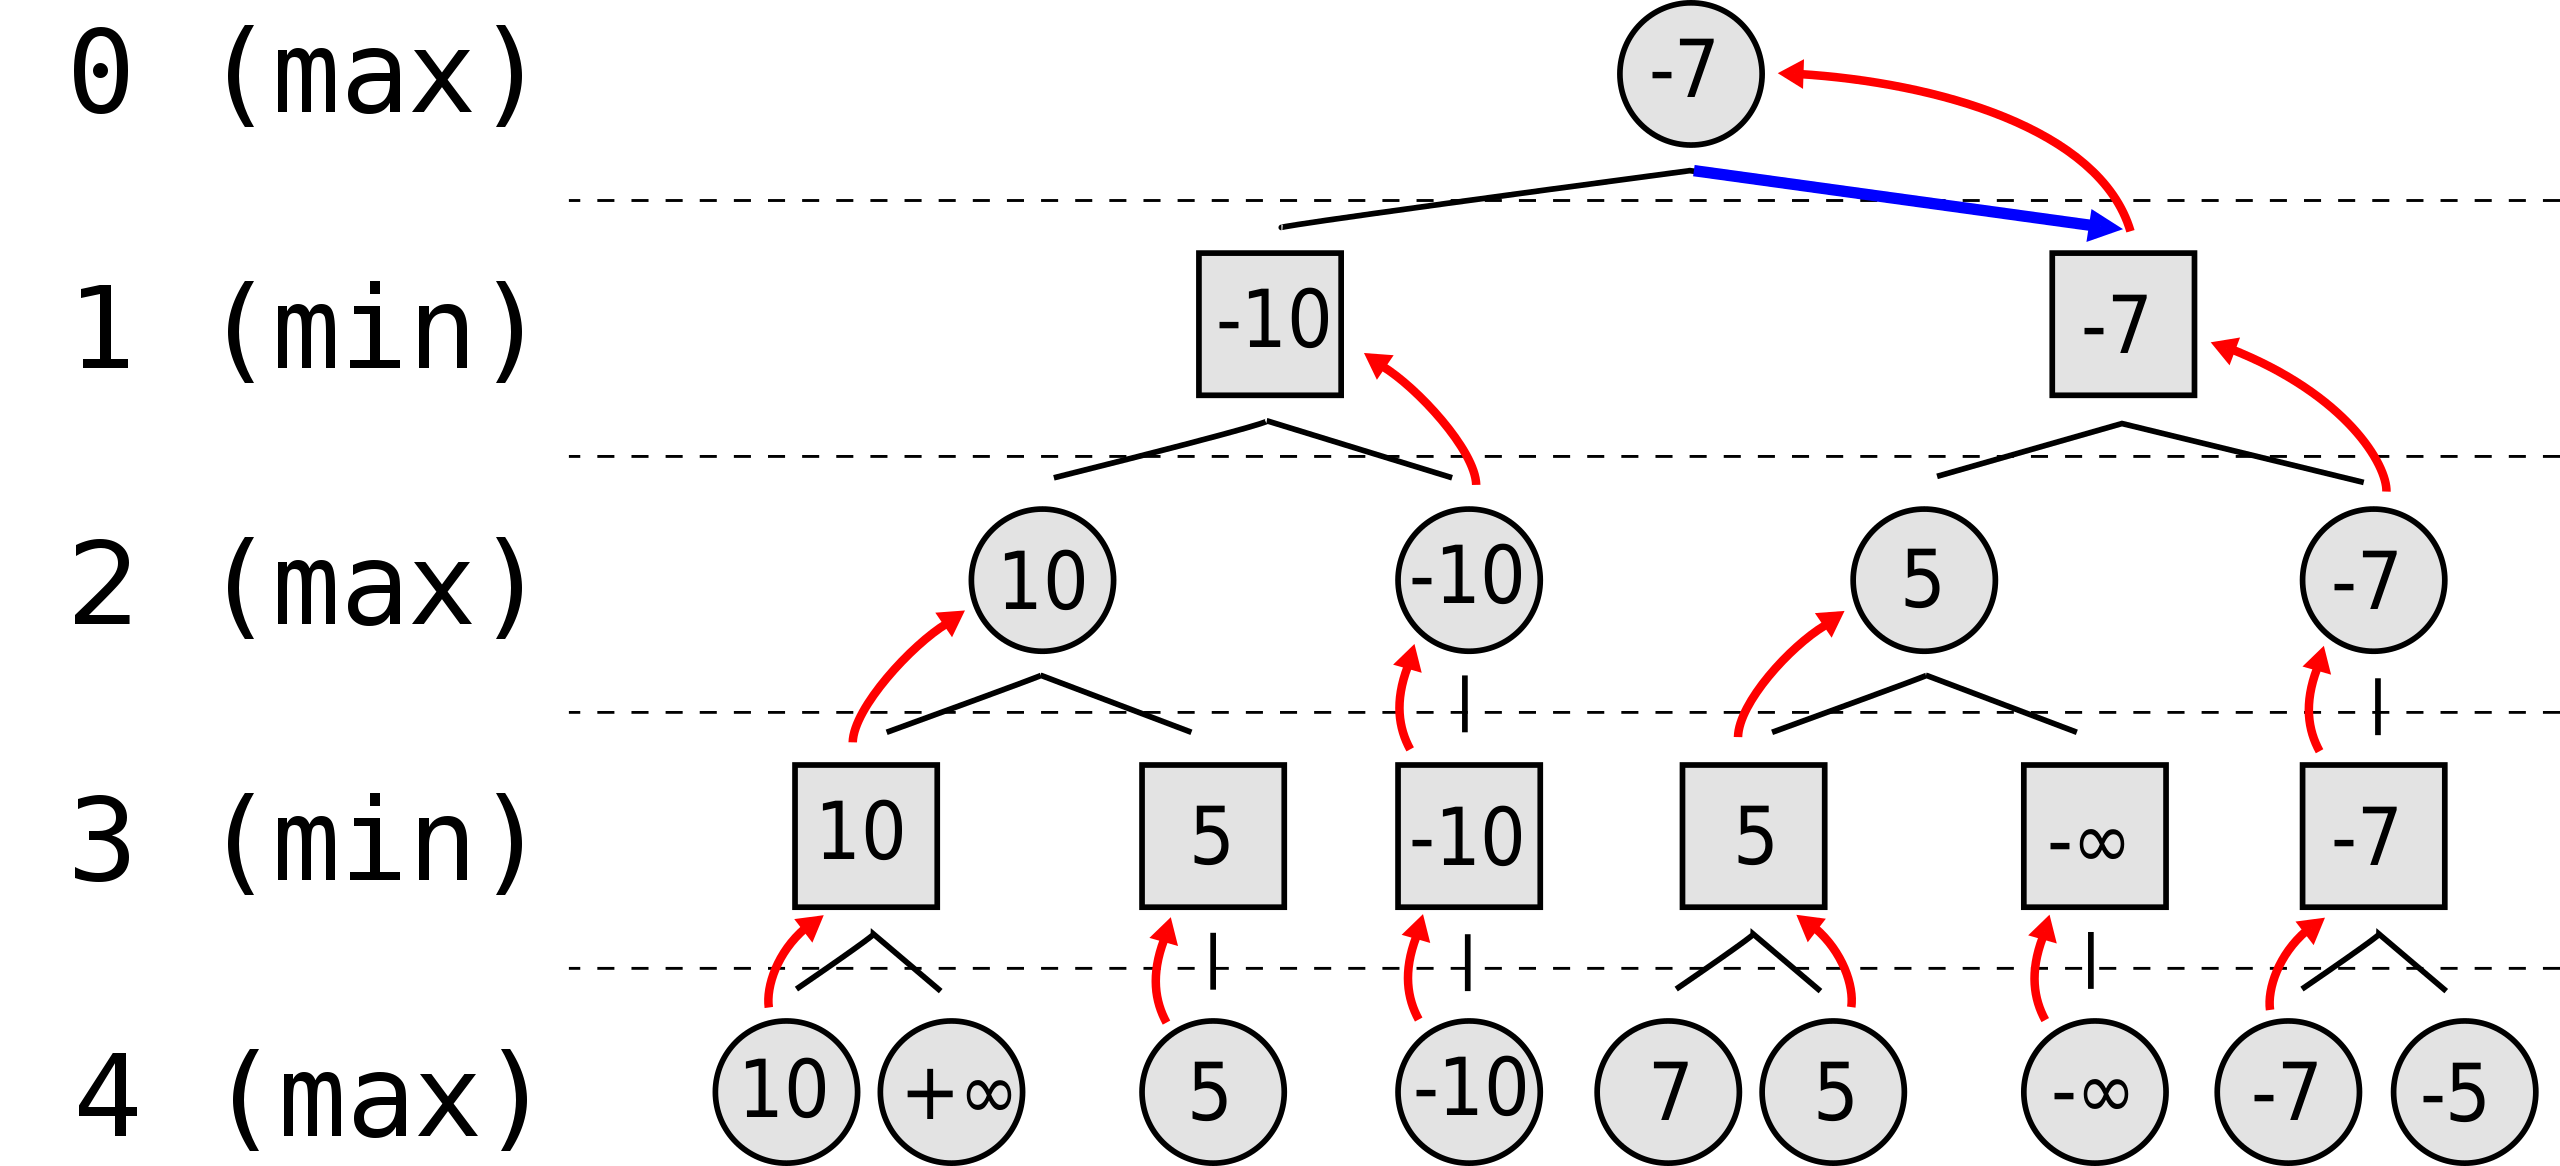
\includegraphics[width=0.6\textwidth]{Minimax.png}
    \caption[minimax]{%
      极小化极大算法搜索树例子\cite{wikiMinimax}%
      }
    \label{fig:superQueenRules}
  \end{figure}

假设圆形代表当前选手,方形代表对手。当前选手需要将自己所得分数最大化,而对手则需要反其道行之。考虑第三层(Min层)对手在最左侧节点的决策,当前选手在第四层有得分为10或正无穷的行动选择,作为对手要做的是最小化这个分数,于是对手根据结果可以反推出应选择得分为10的行动。其余同理。
\subsection{Alpha-beta 剪枝}

\subsection{蒙特卡洛树搜索}

\section{卷积神经网络模型}

\subsection{深度残差网络}

\section{强化学习}

\subsection{基于策略的算法}

\subsection{基于值的算法}